\chapter{UI Overview}
\label{sec:ui_overview}

In this section, the main GUI components are described, to give an overview and introduce the different workflow options.

\subfile{ui_main_window}

\section{Main Menu}
\label{sec:main_menu}

\subsection{File Menu}
\label{sec:ui_overview_file_menu}

Databases can be created, opened and closed using the 'File' menu.

\begin{figure}[H]
  \center
    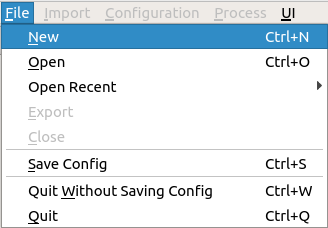
\includegraphics[width=6cm,frame]{figures/ui_file_menu.png}
  \caption{File Menu}
\end{figure}

\begin{itemize}
 \item New: Create new database file
 \item Open: Open existing database file
 \item Open Recent: Open recent existing database file
 \item Export: Create a backup copy of the database file
 \item Close: Close current database
 \item Save Config: Save current configuration
 \item Quit Without Saving Config: Quit application without saving configuration
 \item Quit: Quit application with saving configuration
\end{itemize}
\  \\

After a database was created or opened, the 'Import' menu becomes available.

\subsection{Import Menu}
\label{sec:ui_overview_import_menu}

Data can be imported into the database using the 'Import' menu. This menu is only accessible if a database has been opened.

\begin{figure}[H]
  \center
    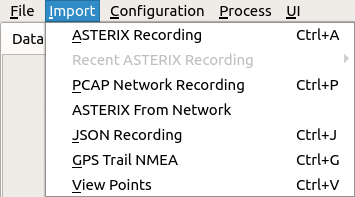
\includegraphics[width=6cm,frame]{figures/ui_import_menu.png}
  \caption{Import Menu}
\end{figure}

\begin{itemize}
 \item ASTERIX Recording: Import ASTERIX recording file
 \begin{itemize}
 \item see \nameref{sec:ui_import_asterix}
 \end{itemize}
 \item PCAP Network Recording: Import ASTERIX from a PCAP network recording
  \begin{itemize}
 \item see \nameref{sec:ui_import_pcap}
 \end{itemize}
 \item ASTERIX From Network: Import ASTERIX from network interfaces in Live mode
  \begin{itemize}
 \item see \nameref{sec:ui_import_asterix_network}
 \end{itemize}
 \item JSON Recording: Import JSON recording file
  \begin{itemize}
 \item see \nameref{sec:ui_import_json}
 \end{itemize}
 \item GPS Trail: Import (D)GPS trail from NMEA file
  \begin{itemize}
 \item see \nameref{sec:ui_import_gps}
 \end{itemize}
 \item View Points: Import View Points definition file
  \begin{itemize}
 \item see \nameref{sec:ui_import_viewpoints}
 \end{itemize}
\end{itemize}
\  \\

\subsection{Configuration Menu}
\label{sec:ui_overview_config_menu}

Data Sources and Sectors can be configured using the 'Configuration' menu. Further, the currently defined Meta Variables can be inspected.

\begin{figure}[H]
  \center
    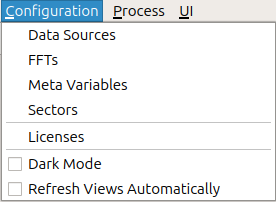
\includegraphics[width=5cm,frame]{figures/ui_configuration_menu.png}
  \caption{Configuration Menu}
\end{figure}

\begin{itemize}
 \item Data Sources: Configure Data Sources
  \begin{itemize}
   \item see \nameref{sec:ui_configure_data_sources}
  \end{itemize}
 \item FFTs: Configure Fixed Field Transponders
  \begin{itemize}
   \item see \nameref{sec:ui_configure_ffts}
  \end{itemize}
 \item Meta Variables: Display current Meta Variables
  \begin{itemize}
   \item see \nameref{sec:configure_meta_vars}
  \end{itemize}
 \item Sectors: Configure Sectors in the database
  \begin{itemize}
   \item see \nameref{sec:ui_configure_sectors}
  \end{itemize}
 \item \nameref{sec:ui_configure_licenses}: Manage licenses
 \item \nameref{sec:ui_overview_dark_mode}: Enable/Disable dark mode (after restart)
 \item Refresh Views Automatically: Sets if views show trigger an automatic data reload process if any configuration changes are made (e.g. adding a DBContent variable in Table View)
\end{itemize}
\  \\ 

\subsection{Process Menu}
\label{sec:ui_overview_process_menu}

Post-processing tasks can be performed using the 'Process' menu. This menu is only accessible if a database was opened.

\begin{figure}[H]
  \center
    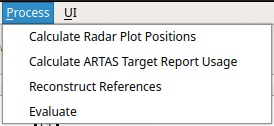
\includegraphics[width=5cm,frame]{figures/ui_process_menu.png}
  \caption{Process Menu}
\end{figure}

\begin{itemize}
 \item \nameref{sec:ui_proc_radar_plot_pos}: (Re-)Calculate Radar plot position information
 \item \nameref{sec:ui_associate_tr_artas}: Associate used target reports to ARTAS tracks based on ARTAS TRI information
 \item \nameref{sec:ui_proc_reconst_references}: Find unique targets, associate target reports and calculate reference trajectories
 \item \nameref{sec:ui_proc_evaluate}: Run a new Evaluation
\end{itemize}
\  \\

\subsection{UI Menu}
\label{sec:ui_overview_ui_menu}

The UI can be reset to a "default" state (as existed at application startup) using the 'Reset Views' function.

\subfile{import/ui_import}
\subfile{config/ui_configuration}
\subfile{process/ui_process}
\subfile{ui_ui}
\subfile{ui_views}

\section{Dark Mode}
\label{sec:ui_overview_dark_mode}

After Dark Mode is enabled or disabled (requiring an application restart), the GUI is switched to a dark theme.

\begin{figure}[H]
  \hspace*{-2.5cm}
    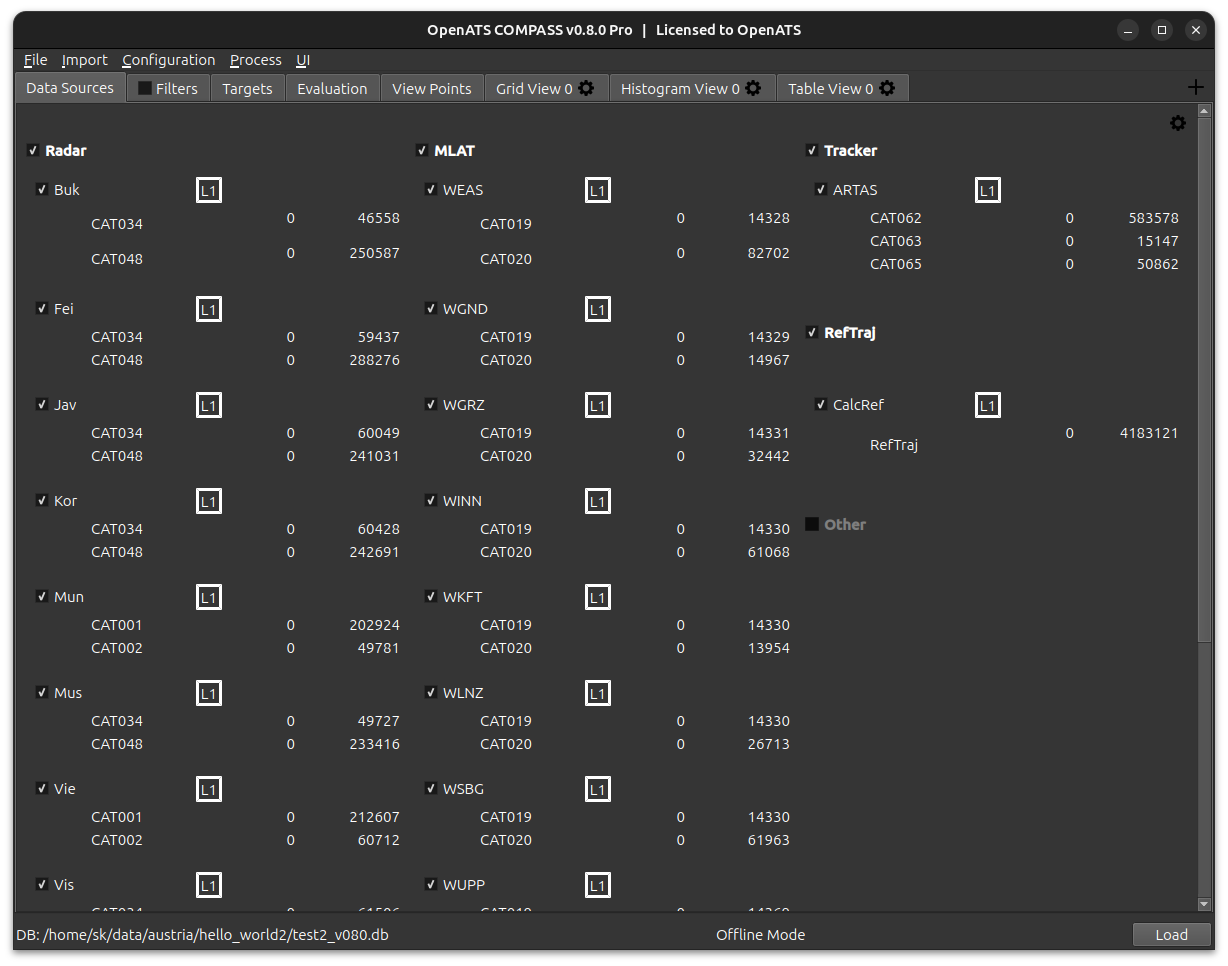
\includegraphics[width=19cm]{figures/dark_mode.png}
  \caption{Main Window Dark Mode}
\end{figure}

Please \textbf{note} that this mode is currently experimental, and not all Views support this dark background color, and some GUI elements may show unexpected coloring. This will be improved in the future. Please also \textbf{note} that the window decoration color can only be changed using your Linux window manager settings. \\

There also exist special dark mode maps for Geographic View as described in \nameref{ref:geoview_map_osm_dark}.

